\chapter{Identity-based Encryption}

Az Identity-based Encryption olyan nyilvános kulcsú titkosítási eljárás, amely esetén a publikus kulcs egy tetszőleges karaktersorozat lehet, amely egyértelműen azonosítani tud egy entitást.

A fejezetben kifejtjük az IBE célját és működését, azonban ezt megelőzően még egy rövid betekintést adunk a párosítások működésébe és fontosságába.

\section{Párosítás-alapú kriptográfia}

A párosítás lényege, hogy egy bizonyos csoporton definiált nehéz probléma átalakítható egy könnyebb problémává egy másik csoport felett. Ez a leképezés számos új kriptográfiai séma létrejöttét tette lehetővé, köztük az Identity-based Encryptionét.

\subsection{A párosítás elterjedése a kriptográfiában}

A párosítás-alapú kriptográfia egy nagyon fiatal terület, mely a párosítások kriptoanalízisben való alkalmazásából fejlődött ki \cite{ReducingEllipticCurveLogarithms}. A MOV redukcióval sikerült szuperszinguláris görbék esetén az elliptikus görbe diszkrét logaritmus problémát redukálni egy véges testen értelmezett diszkrét logaritmus problémává.

A következő lépéseket a párosítás-alapú kriptográfia kialakulása felé Joux tette, aki a Weil és Tate párosításokat használta a Diffie-Hellmann protokoll egy variációjának létrehozására \citeyear{JouxPairingBasedCrypto}.

Ezt követően készítette el Boneh és Franklin a csoportok közti bilineáris leképezésen (például Weil és Tate párosításon) alapuló IBE rendszerüket \citeyear{Boneh::IdentityBasedEncryptionFromTheWeilPairing}. 

Ezeket a munkákat tekinthetjük a párosítás-alapú kriptográfia úttörőinek.

\subsection{A párosítás tulajdonságai}

Az alfejezetben El Mrabet és Joye munkáját vesszük alapul a párosítás tulajdonságainak ismertetéséhez \citeyear{GuideToPairingBasedCrypto}.

Jelöljön $G_1, G_2$ additív, míg $G_\mathbb{T}$ multiplikatív $r$ rendű csoportokat. Az $e$ párosítás egy olyan $e : G_1 \times G_2 \rightarrow G_\mathbb{T}$ leképezés, amely a következő tulajdonágokkal rendelkezik:
\begin{outdentlist}
    \item[] \textbf{Bilineáris.} Jelölje $\mathbb{Z}_r$ az egész számok halmazát modulo $r$, ekkor $\forall P_1 \in G_1, P_2 \in G_2$ és $a, b \in \mathbb{Z}_r$ esetén $e(aP_1, bP_2) = e(P_1, P_2)^{ab}$.

    \item[] \textbf{Nem elfajuló.} Ha $P_1 \neq 0_{G_1}$ és $P_2 \neq 0_{G_2}$, akkor $e(P_1, P_2) \neq 1_{G_\mathbb{T}}$, ahol $0_{G_1}$ (illetve $0_{G_2}$ és $1_{G_\mathbb{T}}$) az egységeleme a $G_1$ csoportnak (illetve $G_2$ és $G_\mathbb{T}$ csoportnak).

    \item[] \textbf{Hatékonyan számítható.}

    \item[] \textbf{Nehezen megfordítható.}
\end{outdentlist}

A kriptográfiában elterjedten használt párosítási módszerek a Weil és a Tate párosítás.

\section{Személyre szabott titkosítás}

Ahogy azt a fejezet elején említettük, az IBE egy olyan nyilvános kulcsú titkosítási eljárás, melynek esetén a publikus kulcs tetszőleges olyan karaktersorozat lehet, amely egyértelműen azonosítani tud egy entitást. Fontos azonban, hogy nemcsak az azonosító, hanem az annak hatókörét jelentő domain is tetszőleges. Lehet csupán néhány fős (például egy vállalat), vagy akár globális kiterjedésű is.

A kitalált séma célja az volt, hogy az entitások kulcscsere nélkül tudjanak egymásnak titkosított üzenetet küldeni \cite{AdiShamirIBE}. Azonban éveken át sikertelenül próbáltak létrehozni jól működő IBE sémákat.

A már említett, Boneh és Franklin \citeyear{Boneh::IdentityBasedEncryptionFromTheWeilPairing} nevéhez fűződő rendszer volt az első, amely teljesen működőképesnek és a gyakorlatban is hatékonyan használhatónak bizonyult.

\subsection{Boneh-Franklin Identity-based Encryption}

Shamir eredeti elképzelése az volt, hogy a publikus kulcsa mindenkinek az email címe legyen. Ennek köszönhetően megspórolhatóvá válna a publikus kulcs megszerzésének költsége.

Az elgondolt séma működése egyszerű. Mikor Kriszta titkosított emailt szeretne küldeni Aladárnak, egyszerűen titkosítja azt Aladár email címével, majd elküldi. Ahhoz, hogy Aladár az üzenetet el tudja olvasni, előbb vissza kell fejtenie. Ezt úgy tudja megtenni, hogy a használt alkalmazás által specifikált módon azonosítja magát, ami után eléri a privát kulcs generátort (PKG). A PKG felelős a felhasználók privát kulcsának elkészítéséért. Az elkészült privát kulcs eljut Aladárhoz, aki azt felhasználva vissza tudja fejteni az üzenetet. Ez a folyamat megtekinthető a \dotref{Figure::ShamirIBE} ábrán.

\begin{figure}[H]
    \centering
    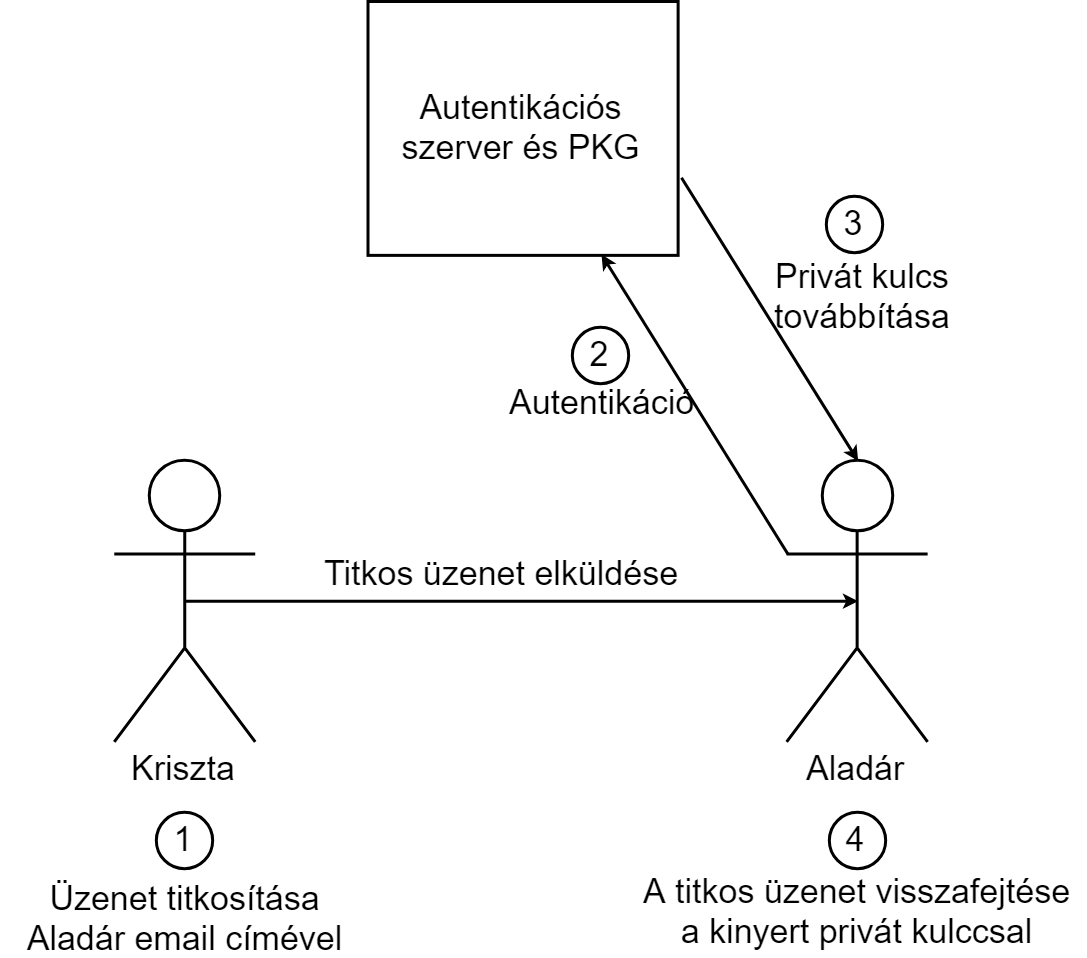
\includegraphics[width=0.6\textwidth]{03-identity-based-encryption/IBE.png}
    \caption{Az IBE működése.}
    \label{Figure::ShamirIBE}
\end{figure}

A séma előbb vázolt működéséhez szükséges még egy, az ábrán nem szereplő előkészítő lépés is. Ennek részeként létrejönnek az úgynevezett publikus paraméterek, valamint a mesterkulcs. Ahhoz, hogy titkosított kommunikációt folytathassunk, először be kell szereznünk a publikus paramétereket; kiemelendő ugyanakkor, hogy erre csak egyszer van szükség, hiszen ezek a paraméterek függetlenek mind a feladótól, mind a címzettől. Míg a publikus paraméterek a rendszer összes felhasználója számára ismertek, addig a mesterkulccsal csupán a PKG rendelkezik  – a privát kulcsok előállítása ugyanis csak ennek birtokában lehetséges.

Boneh és Franklin egy ennek az elképzelésnek eleget tevő rendszert dolgozott ki, amelyet négy algoritmus alkot. Ezek leírásához Martin könyvét \citeyear{Martin::IntroductionToIdentityBasedEncryption} és Kovács diplomamunkáját \citeyear{Kovacs::IBE} vettük alapul.

Az egyes algoritmusok ismertetésének és az azokat követő pszeudokódoknak a megértését elősegíti a \dotref{table::IBEParams} táblázat, amiben összefoglaltuk a különböző paraméterek jelentését.

\begin{table}[H]
    \centering
    \begin{tabular}{|l|l|l|}
        \hline
        \multicolumn{1}{|c|}{\textbf{Paraméter neve}} & \multicolumn{1}{c|}{\textbf{Típusa}} & \multicolumn{1}{c|}{\textbf{Megjegyzés}}              \\ \hline
        $q$                                                  & prím                                 & \multicolumn{1}{c|}{-}                                        \\ \hline
        $p$                                                  & prím                                 & \multicolumn{1}{c|}{-}                                        \\ \hline
        $E(\mathbb{F}_p)$                                     & elliptikus görbe                     & \multicolumn{1}{c|}{-}                                        \\ \hline
        $G_1$                                                & az $E(\mathbb{F}_p)$ ciklikus részcsoportja                     & generátora $P$            \\ \hline
        $G_\mathbb{T}$                                                & az $E(\mathbb{F}_p)$ ciklikus részcsoportja                     & generátora $e(P, P)$        \\ \hline
        $e$                                                  & párosítás                            & $e : G_1 \times G_1 \rightarrow G_\mathbb{T}$                          \\ \hline
        $n$                                                  & egész szám                           & a titkosítatlan szöveg hossza                                 \\ \hline
        $P$                                                  & elliptikus görbe pontja              & $P \in E(\mathbb{F}_p)$                                        \\ \hline
        $sP$                                                 & elliptikus görbe pontja              & $sP \in E(\mathbb{F}_p)$                  \\ \hline
        $H_1$                                                & kriptográfiai hash függvény          & $H_1 : \{0, 1\}^* \rightarrow G_1$                            \\ \hline
        $H_2$                                                & kriptográfiai hash függvény          & $H_2 : G_\mathbb{T} \rightarrow \{0, 1\}^n$                            \\ \hline
        $H_3$                                                & kriptográfiai hash függvény          & $H_3 : \{0, 1\}^n \times \{0, 1\}^n \rightarrow \mathbb{Z}_q$ \\ \hline
        $H_4$                                                & kriptográfiai hash függvény          & $H_4 : \{0, 1\}^n \rightarrow \{0, 1\}^n$                     \\ \hline
    \end{tabular}
    \caption{A Boneh-Franklin Identity-based Encryption paraméterei.}
    \label{table::IBEParams}
\end{table}

\begin{outdentlist}
    \item[]\textbf{Setup.}
    Ez a függvény felelős a rendszer inicializálásáért, a felhasználóhoz tartozó publikus paraméterek és a mesterkulcs előállításáért. Bemenetként a biztonsági fokot meghatározó $k$ paramétert várja. A \dotref{table::RFC::SecurityParam} táblázatban az RFC 5091 ajánlásai láthatók a különböző $k$ értékekre vonatkozóan \cite{RFC5091}. A táblázatban szereplő $k$ értékek a hasonló biztonságot nyújtó RSA kulcshosszak méretét jelképezik, ahogy azt az NSA táblázatából is leolvashatjuk \cite{NSA::EllipticCurve}.

    \begin{table}[H]
        \centering
        \begin{tabular}{|l|l|l|l|}
            \hline
            \multicolumn{1}{|c|}{\textbf{$k$ értéke}} & \multicolumn{1}{c|}{\textbf{$q$ bithosszúsága}} & \multicolumn{1}{c|}{\textbf{$p$ bithosszúsága}} & \multicolumn{1}{c|}{\textbf{Jelölése a dolgozatban}}\\ \hline
            $1024$                           & $160$                                  & $512$                           & LOWEST                                  \\ \hline
            $2048$                           & $224$                                  & $1024$                           & LOW                                 \\ \hline
            $3072$                           & $256$                                  & $1536$                           & MEDIUM                                 \\ \hline
            $7680$                           & $384$                                  & $3840$                           & HIGH                                 \\ \hline
            $15360$                          & $512$                                  & $7680$                           & HIGHEST                                 \\ \hline
        \end{tabular}
        \caption{Az RFC 5091 ajánlásai a biztonsági paraméternek megfelelő bithosszakra.}
        \label{table::RFC::SecurityParam}
    \end{table}

    A \textit{Setup} pszeudokóját az Algoritmus \ref{algorithm:setup} adja meg.

    \begin{algorithm}[H]
        \floatname{algorithm}{Algoritmus}
        \caption{Setup}
        \label{algorithm:setup}
        \begin{algorithmic}
            \Procedure{Setup}{$k$} 
            \State $q$ prím inicializálása \Comment $k$ paraméternek megfelelően
            \State $p$ prím inicializálása \Comment $k$ paraméternek megfelelően
            \State $E(\mathbb{F}_p)$ elliptikus görbe inicializálása
            \State $P = randomPoint(E(\mathbb{F}_p))$ \Comment $P \in E(\mathbb{F}_p)$
            \State $G_1$ csoport generátora legyen $P$
            \State $e : G_1 \times G_1 \rightarrow G_\mathbb{T}$ párosítás kiválasztása
            \State $G_\mathbb{T}$ csoport generátora legyen $e(P, P)$
            \State $s = randomInteger(q)$ \Comment $s \in \mathbb{Z}_q$
            \State $H_1 : \{0, 1\}^* \rightarrow G_1$ kriptográfiai hash függvény kiválasztása
            \State $H_2 : G_\mathbb{T} \rightarrow \{0, 1\}^n$ kriptográfiai hash függvény kiválasztása
            \State $H_3 : \{0, 1\}^n \times \{0, 1\}^n \rightarrow \mathbb{Z}_q$ kriptográfiai hash függvény kiválasztása
            \State $H_4 : \{0, 1\}^n \rightarrow \{0, 1\}^n$ kriptográfiai hash függvény kiválasztása
            \State $PublicParameters = (G_1, G_\mathbb{T}, e, n, P, sP, H_1, H_2, H_3, H_4)$
            \State \Return $s, PublicParameters$ \Comment $s$ a mesterkulcs
            \EndProcedure
        \end{algorithmic}
    \end{algorithm}

    \item[]\textbf{Extract.}
    Az azonosítóhoz tartozó privát kulcs kinyerésére szolgáló függvény. Bemenetként egy $ID$ azonosítót vár. A privát kulcsot csak egyszer kell generálni, aztán mindaddig használható, amíg nem kompromittálódik. Ha egy privát kulcs kompromittálódik, például ellopják, az azt jelenti, hogy minden üzenet, ami az ahhoz tartozó nyilvános paraméterekkel lett titkosítva, veszélyben van. A séma nem ad támogatást ilyen veszéllyel szemben, azonban a \textit{Setup} függvény újrafuttatásával új nyilvános paraméterek generálhatók, ekképpen az új üzenetek ismét biztonságban lehetnek.
    \begin{algorithm}[H]
        \floatname{algorithm}{Algoritmus}
        \caption{Extract}
        \label{algorithm:extract}
        \begin{algorithmic}
            \Procedure{Extract}{$ID$} 
            \State $Q_{ID} = H_1(ID)$
            \State \Return $sQ_{ID}$
            \EndProcedure
        \end{algorithmic}
    \end{algorithm}

    \item[]\textbf{Encrypt.}
    Az üzenet titkosítását végző függvény. Bemenetként egy $M$ üzenetet és egy $ID$ azonosítót vár.
    \begin{algorithm}[H]
        \floatname{algorithm}{Algoritmus}
        \caption{Encrypt}
        \label{algorithm:encrypt}
        \begin{algorithmic}
            \Procedure{Encrypt}{$M, ID$} 
            \State $Q_{ID} \gets H_1(ID)$
            \State $\sigma \gets randomBits(n)$ \Comment $\sigma \in \{0, 1\}^n$
            \State $r \gets H_3(\sigma, M)$
            \State $C_1 \gets rP$
            \State $C_2 \gets \sigma \oplus H_2(e(rQ_{ID}, sP))$
            \State $C_3 \gets M \oplus H_4(\sigma)$
            \State $C \gets (C_1, C_2, C_3)$
            \State \Return {$C$}
            \EndProcedure
        \end{algorithmic}
    \end{algorithm}

    \item[]\textbf{Decrypt.}
    A titkos üzenet visszafejtéséért felelős függvény. Bemenetként egy $C$ titkos üzenetet és egy $sQ_{ID}$ privát kulcsot vár.
    \begin{algorithm}[H]
        \floatname{algorithm}{Algoritmus}
        \caption{Decrypt}
        \label{algorithm:decrypt}
        \begin{algorithmic}
            \Procedure{Decrypt}{$C, sQ_{ID}$} 
            \State $\sigma \gets C_2 \oplus H_2(e(sQ_{ID}, C_1))$
            \State $M \gets C_3 \oplus H_4(\sigma)$
            \State $r = H_3(\sigma, M)$
            \If {$C_1 \neq rP$} 
                \State \Return {error} \Comment Hibás bemenet.
            \EndIf
            \State \Return {$M$}
            \EndProcedure
        \end{algorithmic}
    \end{algorithm}
\end{outdentlist}

Fontos megjegyezni, hogy az \textit{Encrypt} és \textit{Decrypt} függvények egymás inverzét alkotják. Ez azt jelenti, hogy ha $\mathcal{M}$ jelöli az üzenetteret, akkor $\forall M \in \mathcal{M} :$ \textit{Decrypt}(\textit{Encrypt}($M$, $ID$), $sQ_{ID}$) $= M$ \cite{Boneh::IdentityBasedEncryptionFromTheWeilPairing}.

A bizonyítás a párosítás alapvető tulajdonságát használja ki, mely szerint:
$$e(rQ_{ID},sP)=e(Q_{ID},P)^{rs}=e(sQ_{ID},rP).$$
